\chapter{Normalisierung}
\section{Rasterisierung}

\begin{wrapfigure}{R}{0.4\textwidth}
  \vspace{-20pt}
  \begin{center}
    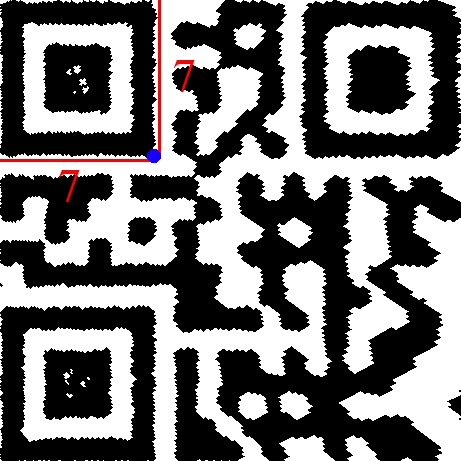
\includegraphics[scale=0.25]{images/Gitter_step.png}
  \end{center}
  \vspace{-10pt}
  \label{fig:raster-qrcode}\caption{Raster}
  \vspace{-10pt}
\end{wrapfigure}

Nach der perspektivischen Transformation, liegt das Bild in einem $n\times n$ großem binärisiertem Zustand vor. Nun muss der \QRCode rasterisiert werden. 
Man betrachte dazu die untere rechte Ecke des oberen linken Finder Pattern. Es ist bekannt, dass ein Finder Pattern die Dimension $7 \times 7$ hat,
sodass man die $x$ bzw. $y$-Koordinate der genannten Ecke durch $7$ dividiert.

Dies liefert die Zellenlänge $z$ des Rasters,
woraus sich die Anzahl der Module $m$ via Division von $n$ mit $z$ berechnen lässt. Im Normalfall gilt jedoch $m \notin \mathbb{Z}$.
Es ist jedoch bekannt, dass ein \QRCode nur 
\begin {equation}
	17 + 4 \cdot version,
\end{equation}
für $version \in \left\{1, ..., 40\right\} \subset \mathbb{N}$, Module besitzen kann.

\todo{Quelle angeben!}
\begin{figure}[h]
\centering
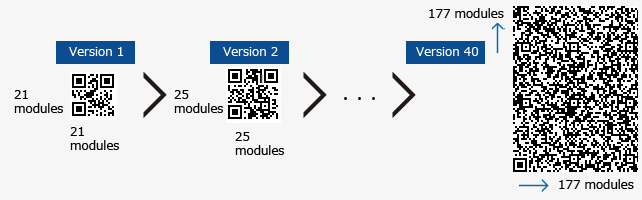
\includegraphics[scale=0.5]{images/QRVersion.png}
\label{fig:version-qrcode}\caption{Mögliche Modulgrößen von QR-Codes}
\end{figure}

Man runde die Anzahl der berechneten Module $m$ auf die nächstliegende Versionsnummer via
\begin{equation}
	version = cvRound((m-17)/4);
\end{equation}
Die zugehörige Anzahl der Module ist dann also gegeben durch
\begin{equation}
	modules = 17+4 \cdot version;
\end{equation} 
Die Zellenlänge des Rasters ist letztendlich gegeben durch Divison von $n$ mit $modules$.

\section{Normalisierung}
Die Normalisierung wird mithilfe des Rasters durchgeführt, indem majority votes pro Zelle den Pixelwert des normalisierten \QRCodes festlegen.
Das Ergebnis ist also ein $modules \times modules$ großer normalisierter \QRCode.
\begin{figure}[h]
\centering
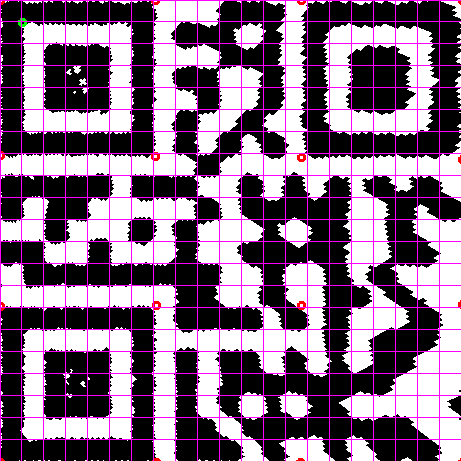
\includegraphics[scale=0.25]{images/gitter.png}
\label{fig:version-qrcode}\caption{Normalisierung des \QRCode}
\end{figure}

\section{Verifikation}
Um fälschlicherweise erkannte \QRCodes vorzubeugen, wird im Anschluss noch eine Verifikation durchgeführt. Dies geschieht, indem die Pixel des normalisierten Bildes, an denen die Finder Patterns und timing Patterns liegen mit den Finder bzw. timing Patterns eines Standard \QRCodes verglichen werden.
\begin{figure}[h]
\centering
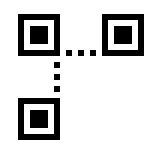
\includegraphics[scale=0.5]{images/verifikation.png}
\label{fig:version-qrcode}\caption{Finder und Timing Patterns eines Standard \QRCode}
\end{figure}

Ist die Übereinstimmung des normalisierten Bildes mit einem Standard \QRCode geringer als $85\%$, so wiederhole die Normalisierung und die Verifikation, falls möglich, mit einer Versionsnummer von $\pm 1$, um falsche Rundungen bei der Rasterisierung vorzubeugen.

Sind alle Übereinstimmungen unter $65\%$, so wird der \QRCode verworfen, andernfalls wird der \QRCode mit der höchsten Übereinstimmung gewählt und schlussendlich ausgegeben.
